\chapter{Plataforma de desarrollo}
\label{cap:capitulo3}

\vspace{1cm}

En este capítulo, se introducen y describen las herramientas, tanto hardware como software, usadas para el desarrollo de este trabajo.

\section{Raspberry Pi 4 Model B}
\label{sec:rpi}

La Raspberry Pi 4 Model B (Figura \ref{fig:raspberry2}) es la plataforma hardware de bajo coste escogida para este proyecto. Debido a la gran comunidad de desarrolladores y usuarios que posee, además de las especificaciones ofrecidas (Cuadro \ref{cuadro:especificaciones_rpi4}) por su escaso precio (65,44 \euro\footnote{Distribuidor oficial de Raspberry: \url{https://www.kubii.es/40-raspberry-pi-3-2-b}}), es la plataforma más usada por la mayoría del público.\\

\begin{figure} [h!]
  \begin{center}
    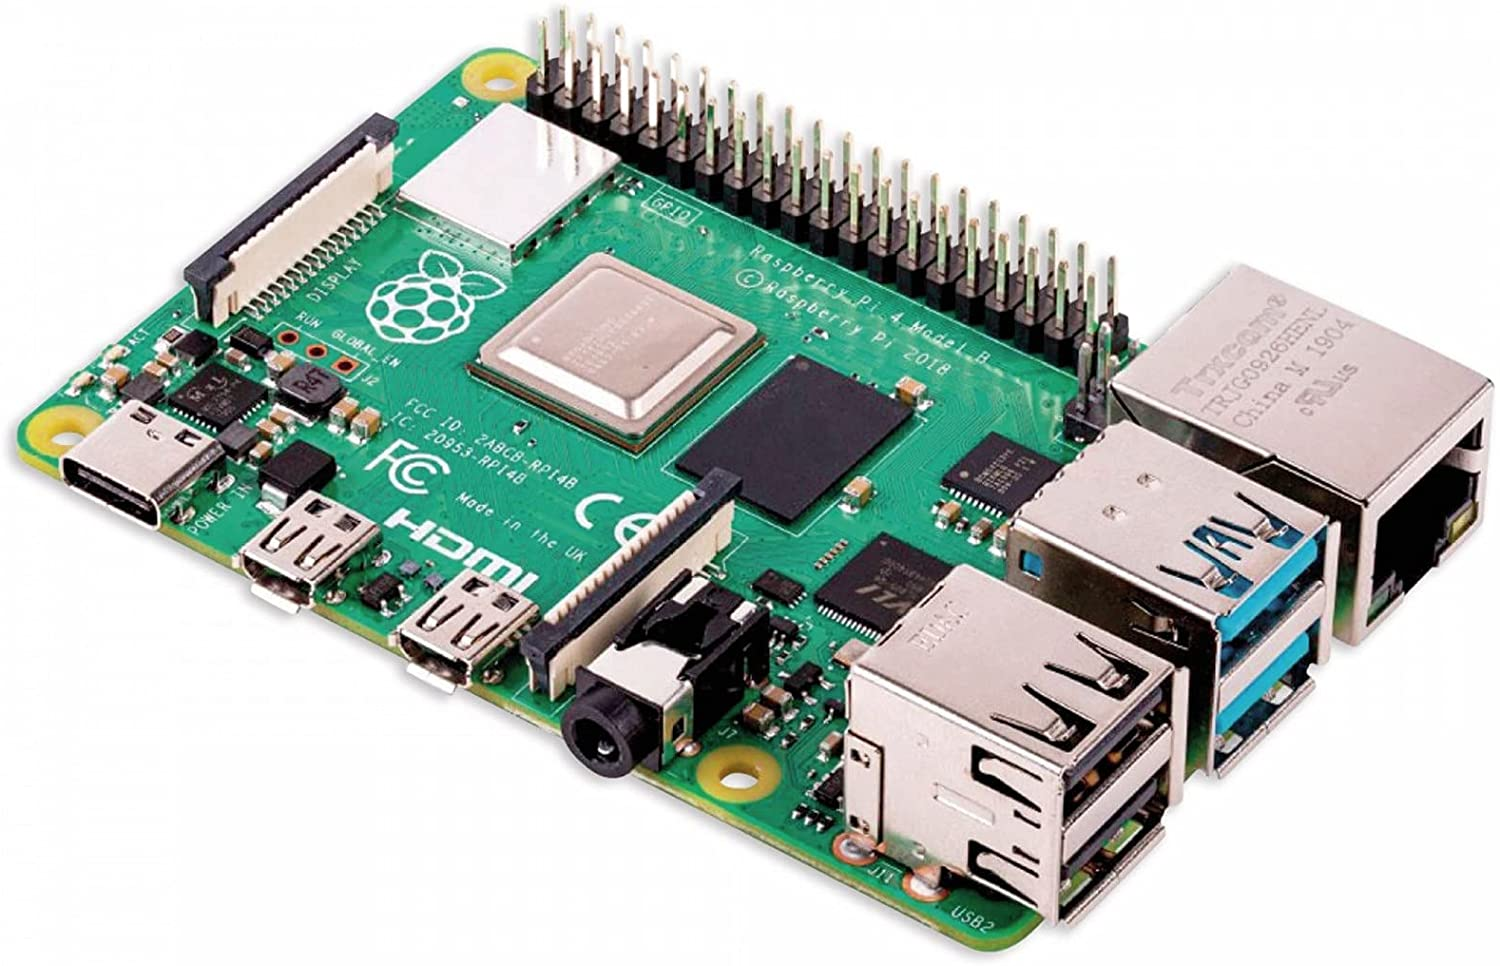
\includegraphics[width=9cm]{figs/raspberry.jpg}
  \end{center}
  \caption{Raspberry Pi 4b.}
  \label{fig:raspberry2}
\end{figure}

Sus características más atractivas ---entre otras--- son su bajo consumo energético, su pequeño tamaño y por lo tanto mínimo peso, su alta conectividad y puertos (red WIFI, Bluetooth, Ethernet, USB2 y USB3, HDMI, etc.) y la gran fluidez que posee su sistema operativo (Sección \ref{sec:raspberry_pi_os}). Todo esto la convierte en una auténtica joya y son cada vez más usuarios los que la utilizan en diversos proyectos. Podemos encontrarla ---por ejemplo--- como centro doméstico inteligente para controlar la domótica de una casa o incluso en sectores más profesionales formando parte de la arquitectura de algunos robots. Esto último es lo más interesante, para nosotros, dentro de los múltiples usos que tiene una Raspberry.\\

\begin{table}[H]
\begin{center}
\begin{tabular}{|>{\arraybackslash}m{3cm} | >{\arraybackslash}m{6cm} |}
     \hline
     Procesador & Broadcom BCM2711 (4 núcleos Cortex-A72 (ARM v8), 64-bit, 1.5Ghz) \\ \hline
     Tarjeta gráfica & Broadcom VideoCore VI (integrada en el procesador) \\ \hline
     Memoria RAM & 4 GB LPDDR4-3200 SDRAM \\ \hline
     \multirow{3}{*}{Conexión}& WIFI 2.4 GHz y 5 GHz\\
     & Bluetooth 5.0/BLE\\
     & Gigabit Ethernet \\ \hline
     \multirow{5}{*}{Puertos}& 2 x micro-HDMI (4K 60 Hz)\\
     & MIPI Display Serial Interface \\
     & MIPI Camera Serial Interface \\
     & Jack Audio/Vídeo \\
     & Slot para micro-SD \\ \hline
     \multirow{2}{*}{Alimentación} & 5V por USB-C (3A mínimo) \\
     & 5V por GPIO (3A mínimo) \\ 
     \hline
 \end{tabular}
\caption{Especificaciones técnicas de la Raspberry Pi 4 Model B.}
\label{cuadro:especificaciones_rpi4}
\end{center}
\end{table}

Muchos de los robots son de tamaño reducido y no tienen el espacio suficiente como para acoplar una gran estación de procesamiento, por lo tanto en esos casos es muy común usar algún modelo de Raspberry como unidad central. Incluso en robots grandes se suelen utilizar también para realizar el control de zonas concretas, por ejemplo de los ojos de un humanoide. Por lo tanto, nuestro sistema de detección de emociones corriendo en la Raspberry Pi 4 Model B puede servir de gran ayuda a la hora de construir uno de estos robots comentados anteriormente que sólo tienen la capacidad de albergar una placa de tamaño reducido, o que simplemente los desarrolladores de dicho robot quieren ahorrar dinero en costes.

\subsection{Raspberry Pi OS}
\label{sec:raspberry_pi_os}

Raspberry Pi OS (Figura \ref{fig:captura_rpios}) es el sistema operativo oficial para Raspberry. Es un sistema operativo gratuito basado en Debian optimizado específicamente para el hardware de la Raspberry Pi, por lo tanto es el que mayor rendimiento nos ofrecerá frente a otros como Ubuntu (que también puede ser instalado). Además, está en constante desarrollo y continuamente se está mejorando su estabilidad y funcionalidad. Es por todo ello que será el sistema operativo elegido en nuestro proyecto, sobre todo por su alto rendimiento (algo esencial para impulsar el desempeño de nuestro sistema de detección de emociones).\\

\begin{figure} [h!]
  \begin{center}
    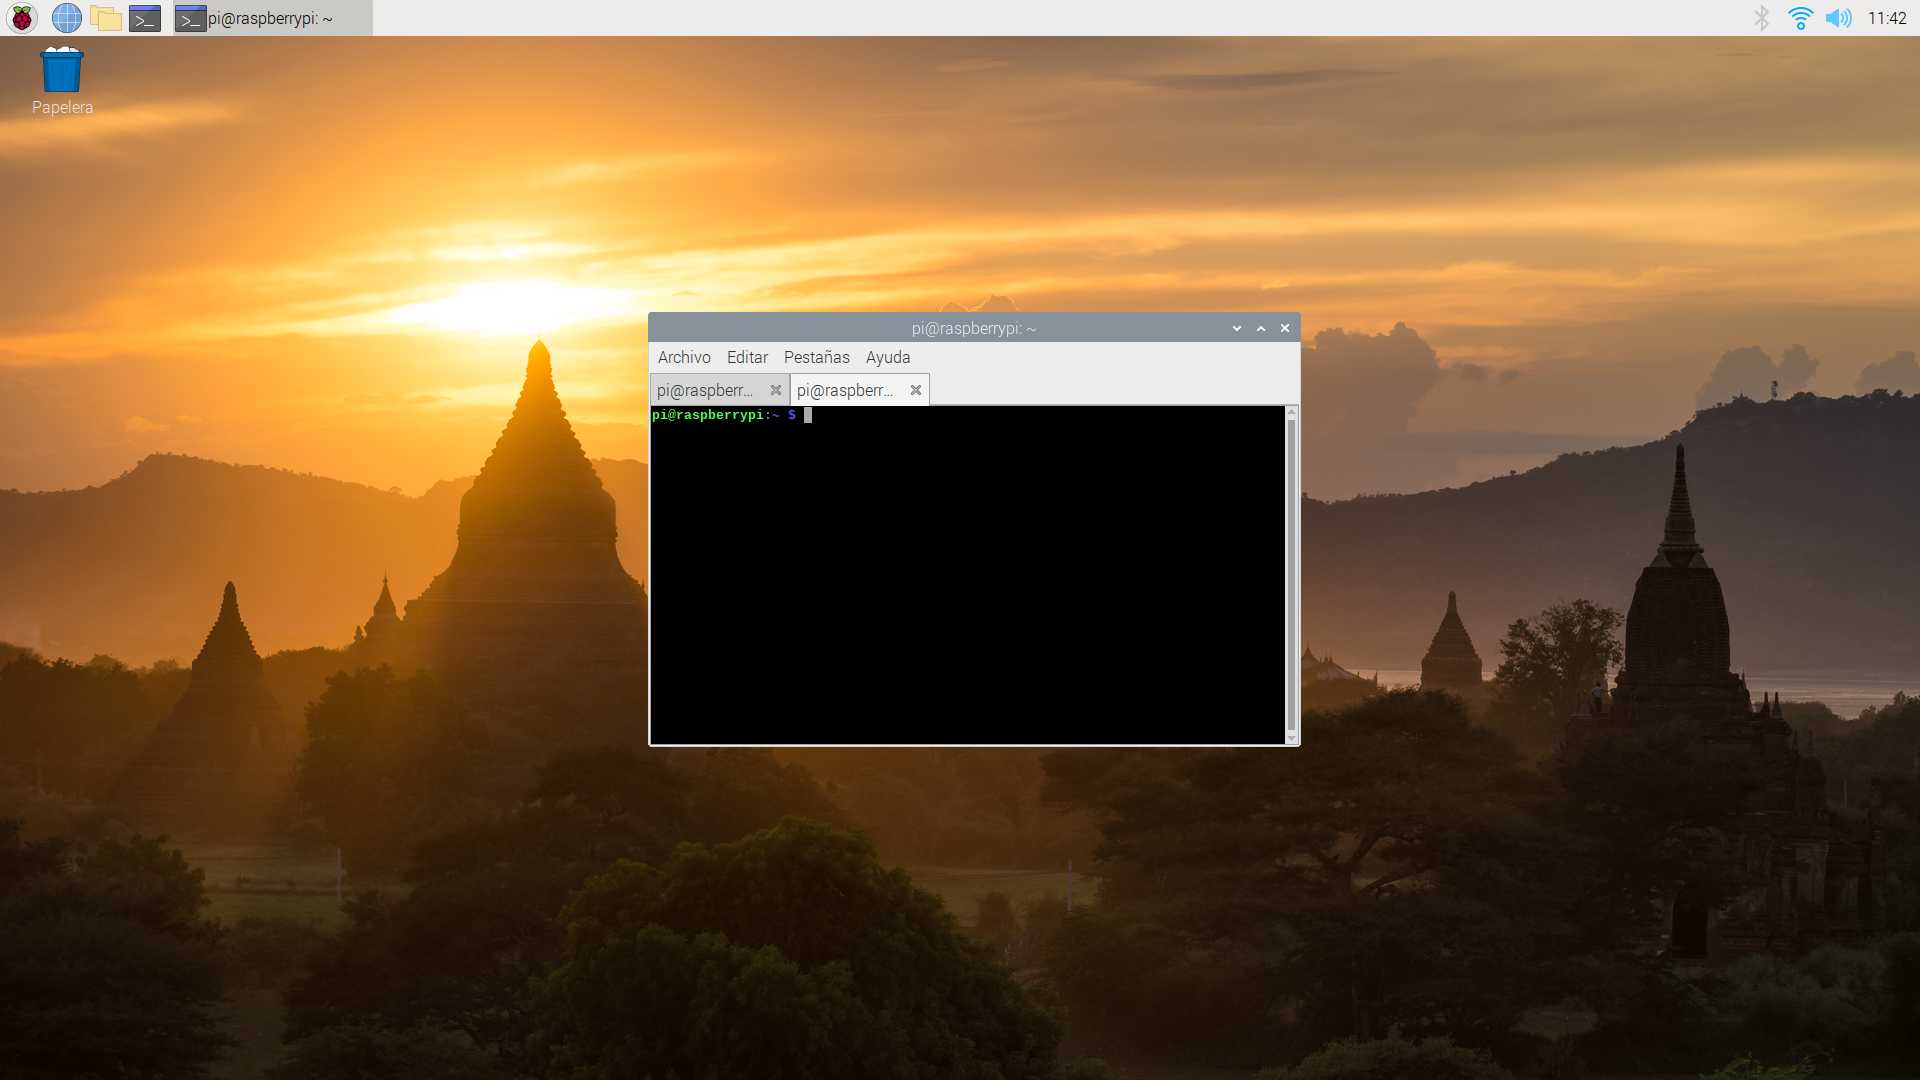
\includegraphics[width=13cm]{figs/captura_rpios.png}
  \end{center}
  \caption{Captura de pantalla de Raspberry Pi OS.}
  \label{fig:captura_rpios}
\end{figure}

La versión de Raspberry Pi OS escogida ha sido Raspberry Pi OS Legacy (Cuadro \ref{cuadro:especificaciones_rpios}). Se ha elegido dicha versión porque, de todas las disponibles, ha sido la única en la que se ha conseguido instalar una versión de ROS/ROS2 (en concreto, ROS Noetic). Además, aunque las versiones de Raspberry Pi OS de 64-bit ofrecían más rendimiento, todavía no estaban maduras y no ofrecían total compatibilidad con todas las librerías usadas en el presente trabajo.

\begin{table}[H]
\begin{center}
\begin{tabular}{|>{\arraybackslash}m{4cm} | >{\arraybackslash}m{4cm} |}
     \hline
     Fecha de lanzamiento & 4 de Abril de 2022 \\ \hline
     Sistema & 32-bit \\ \hline
     Versión del Kernel & 5.10 \\ \hline
     Versión de Debian & 10 (buster) \\ \hline
 \end{tabular}
\caption{Especificaciones de Raspberry Pi OS Legacy.}
\label{cuadro:especificaciones_rpios}
\end{center}
\end{table}

\subsection{Raspberry Pi Camera Module V2.1}
\label{sec:rpi_camera}

La Raspberry Pi Camera (Figura \ref{fig:rpi_camera}) es la cámara oficial desarrollada por Raspberry para ser utilizada en sus placas. Para este trabajo, se ha hecho uso de la versión 2.1 (Cuadro \ref{cuadro:especificaciones_rpi_camera}). Es una cámara de alta definición (3280x2464) que se conecta a cualquier Raspberry Pi compatible a través de una interfaz de bus CSI-2. Además de vídeo de alta calidad, ofrece una reducción de la contaminación de la imagen (ruido o manchas).\\

\begin{figure} [h!]
  \begin{center}
    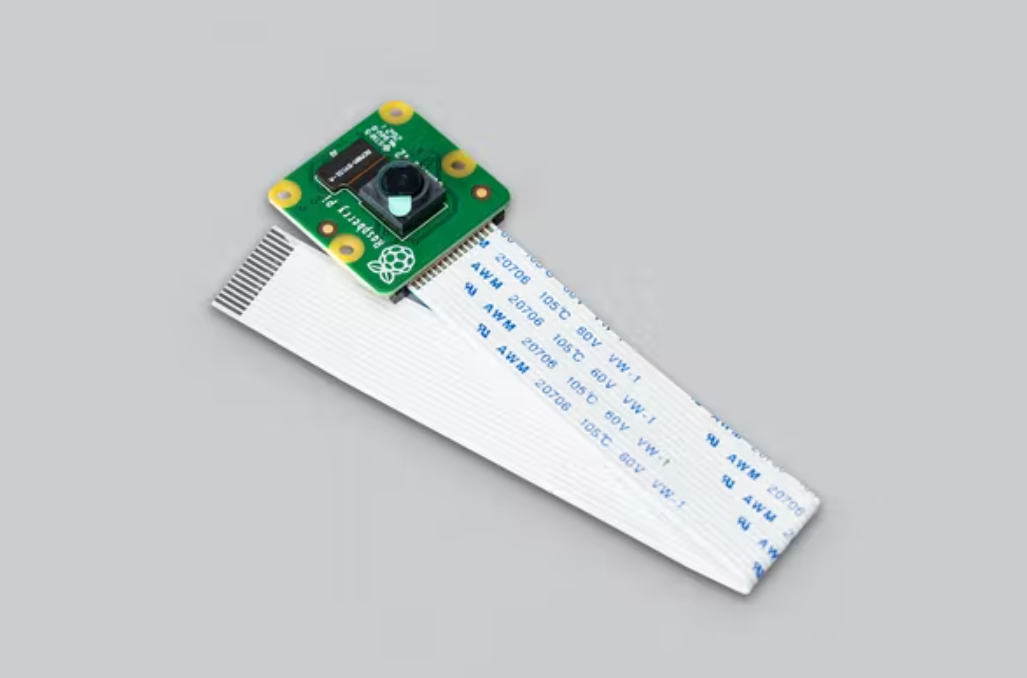
\includegraphics[width=9cm]{figs/rpi_camera.png}
  \end{center}
  \caption{Raspberry Pi Camera Module V2.1.}
  \label{fig:rpi_camera}
\end{figure}

\begin{table}[H]
\begin{center}
\begin{tabular}{|>{\arraybackslash}m{4cm} | >{\arraybackslash}m{6cm} |}
     \hline
     Sensor de imagen & Sony IMX 219 PQ CMOS \\ \hline
     Resolución de imagen & 3280x2464 (8-megapixeles) \\ \hline
     \multirow{2}{*}{Resolución de vídeo}& 1080p 30fps\\
     & 720p 60fps \\ \hline
     Conexión & Cable plano de 15 pines, MIPI Camera Serial Interfaze (CSI-2)\\ \hline
     Peso & 3g \\ \hline
     Dimensiones & 23.86 x 25 x 9 mm \\ \hline 
 \end{tabular}
\caption{Especificaciones de Raspberry Pi Camera Module V2.1.}
\label{cuadro:especificaciones_rpi_camera}
\end{center}
\end{table}

Se ha decidido escoger la Raspberry Pi Camera Module V2.1 en vez de una versión convencional de WebCam (USB) debido a las siguientes ventajas:

\begin{itemize}
    \item \textit{Mayor framerate.} Gracias a que la Raspberry Pi 4 Model B tiene un puerto dedicado para conectar la Raspberry Pi Camera (Figura \ref{fig:rpi_camera_CSI}), es posible conseguir una gran velocidad de fotogramas. Esto es debido a que esa conexión especial permite que la codificación vaya dirigida directamente a la GPU y sólo haya un pequeño impacto en la CPU, dejándola libre para otros usos. En cambio, una WebCam conectada por USB utiliza directamente la CPU, y mover datos a través de un USB es bastante costoso para un sistema de recursos limitados.
    
    \begin{figure} [h!]
      \begin{center}
        \includegraphics[width=9cm]{figs/rpi_camera_CSI.JPG}
      \end{center}
      \caption{MIPI Camera Serial Interfaze (CSI-2).}
      \label{fig:rpi_camera_CSI}
    \end{figure}
    
    \item \textit{Mayor calidad de imagen.} Es cierto que también existen WebCam con una calidad de imagen muy buena, pero su precio es elevado. Por lo tanto, la Raspberry Pi Camera acaba ganando en cuanto a calidad de imagen si realizamos la comparativa en el mismo rango de precio (29,14 \euro\footnote{Distribuidor oficial de Raspberry: \url{https://www.kubii.es/318-camaras-sensores}}). Sin embargo, este no es un apartado muy relevante porque finalmente en el sistema de detección de emociones no hacemos uso de la máxima resolución para aumentar el rendimiento.
    
    \item \textit{Menor tamaño.} El tamaño tan compacto de la Raspberry Pi Camera es uno de sus mayores atractivos y es por eso que es también una gran ventaja frente a las WebCam. De cara a instalar estos pequeños ordenadores con cámara en un robot es esencial que ocupen el menor espacio posible, además de que su peso sea muy reducido.
\end{itemize}

\section{Python}

Python es un lenguaje de programación interpretado (se ejecuta sin necesidad de ser compilado) y de tipado dinámico (las variables se comprueban en tiempo de ejecución). Es de licencia totalmente libre y soporta programación orientada a objetos. Se caracteriza por hacer uso de una sintaxis muy legible en la que es obligatoria una correcta tabulación\\

Se ha escogido Python (versión 3.7.3) como lenguaje de programación para este proyecto debido a los dos siguientes motivos:

\begin{enumerate}
    \item El sistema desarrollado en este trabajo usa algoritmos de Machine Learning para detectar las emociones faciales y Python es el lenguaje de programación rey en ese campo, posee múltiples librerías como Pandas, TensorFlow, Keras, Scikit-learn... que brindan un soporte excepcional para cualquier tarea relacionada con el aprendizaje automático.
    
    \item La librería que da soporte oficial a la Raspberry Pi Camera (Sección \ref{sec:rpi_camera}) únicamente se puede usar en Python. Se trata del paquete \textit{picamera}.
\end{enumerate}

\section{MediaPipe}
\label{sec:mediapipe}

MediaPipe\footnote{MediaPipe: \url{https://mediapipe.dev/}} es una plataforma, perteneciente a Google, que ofrece soluciones open source (código libre) de Machine Learning para varias plataformas: Android, iOS, C++, Python, Javascript y Coral. Se caracteriza por ofrecer algoritmos muy rápidos capaces de funcionar, con valores altos de FPS, sin hacer uso de una GPU. Se puede encontrar el código de todas las herramientas que ofrece en su repositorio\footnote{Repositorio MediaPipe: \url{https://github.com/google/mediapipe}} de GitHub.

\subsection{Face Mesh}

MediaPipe Face Mesh\footnote{MediaPipe Face Mesh: \url{https://google.github.io/mediapipe/solutions/face_mesh}} es una de las soluciones que nos ofrece MediaPipe. Se trata de una herramienta que detecta una malla facial 3D compuesta por 468 puntos usando únicamente una cámara (Figura \ref{fig:mediapipe}). Haremos uso de este sistema en este trabajo para obtener información, en forma de coordenadas, de puntos faciales característicos.\\

\begin{figure} [h!]
  \begin{center}
    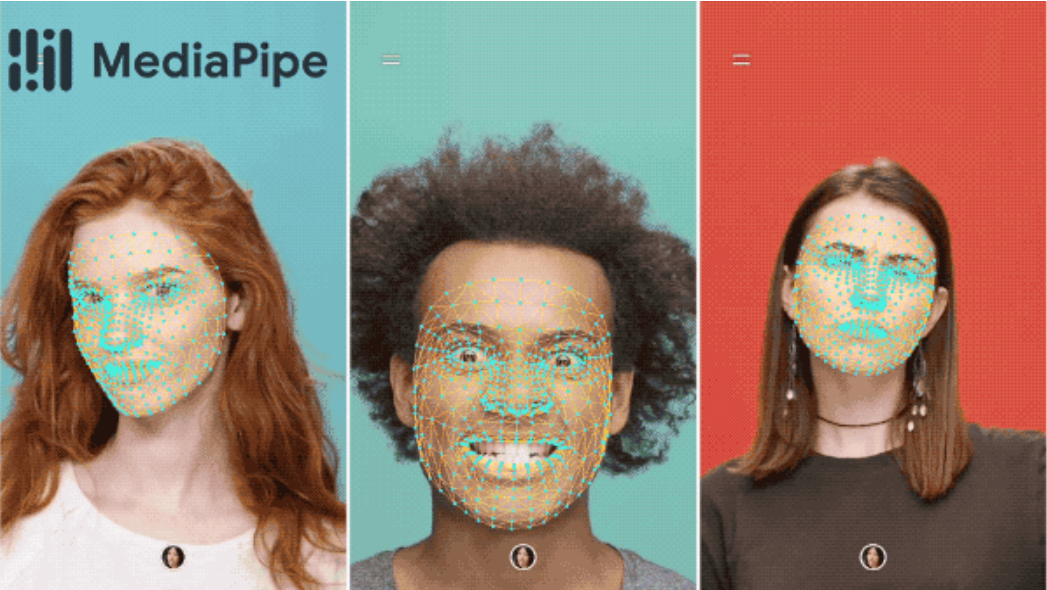
\includegraphics[width=12cm]{figs/mediapipe.png}
  \end{center}
  \caption{Malla facial de MediaPipe.}
  \label{fig:mediapipe}
\end{figure}

La arquitectura de Face Mesh está compuesta por dos modelos de Machine Learning (redes neuronales profundas): un detector facial y otro que predice la superficie 3D de puntos faciales usando únicamente el sector de las caras detectadas, este último desarrollado en el artículo \cite{facemesh_surface}. Tener la cara recortada previamente aumenta el rendimiento. Además, una vez que se han detectado los rostros y se han localizado los puntos de referencia faciales, en los siguientes fotogramas simplemente se procede a realizar un rastreo de dichos puntos en vez de realizar constantemente detecciones (faciales o de coordenadas). Una vez que se pierdan, ya sí que se lleva a cabo una nueva detección.\\

La herramienta posee los siguientes parámetros de entrada que permiten personalizar su funcionamiento:
\begin{itemize}
    \item \verb|static_image_mode|: se indica con un booleano (\textit{True} o \textit{False}) si se va a procesar una imagen estática o un vídeo, para que en caso de que sea un vídeo, realizar las optimizaciones oportunas.
    
    \item \verb|max_num_faces|: se indica con un número entero el número de caras que se desean detectar como máximo.
    
    \item \verb|refine_landmarks|: aumenta la precisión de las coordenadas alrededor de los ojos y los labios, a cambio de un poco más de cómputo. Se activa o desactiva con un booleano (\textit{True} o \textit{False}).
    
    \item \verb|min_detection_confidence|: con un valor del intervalo [0.0, 1.0] se indica al modelo de detección de rostros el valor mínimo de confianza para considerar una predicción exitosa.
    
    \item \verb|min_tracking_confidence|: con un valor del intervalo [0.0, 1.0] se indica al modelo de puntos faciales el valor mínimo de confianza para considerar que los puntos han sido rastreados correctamente.
\end{itemize}

La salida que nos proporciona exactamente el sistema Face Mesh de Mediapipe es una colección de rostros, donde cada rostro se representa como una lista de 468 puntos y cada uno de esos puntos se compone de las variables \textit{x}, \textit{y} y \textit{z}. Las variables \textit{x} e \textit{y} están normalizadas entre 0 y 1, por el ancho y alto de la imagen. La variable \textit{z} contiene la profundidad del punto, siendo el origen el centro de la cabeza.

\section{Detector de puntos faciales. Dlib.}
\label{sec:dlib}

Dlib es un conjunto de herramientas que contiene algoritmos de Machine Learning. En este trabajo se ha hecho uso del detector de puntos faciales, capaz de detectar 68 puntos de referencia, contenido en dlib (Figura \ref{fig:dlib_example}).\\

\begin{figure} [h!]
  \begin{center}
    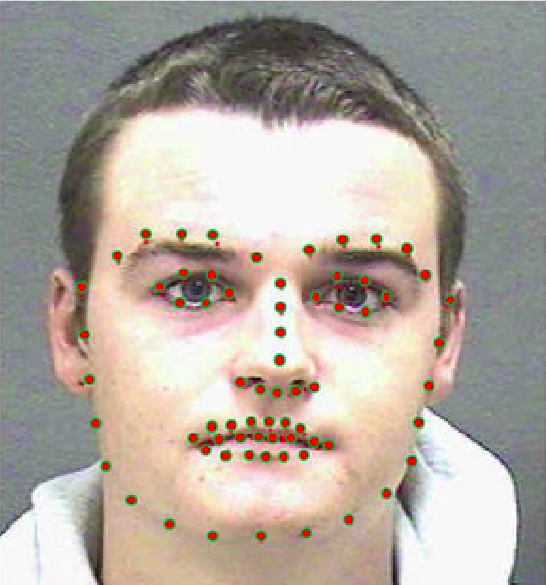
\includegraphics[width=7cm]{figs/dlib_example.png}
  \end{center}
  \captionsetup{justification=centering}
  \caption{Ejemplo usando el detector de puntos faciales de dlib.\\
  Imagen obtenida del artículo \cite{dlib_example}}
  \label{fig:dlib_example}
\end{figure}

El algorimo está compuesto de dos fases: detección del rostro y detección de las regiones faciales. Para realizar la detección de rostros, dlib incluye dos opciones:

\begin{itemize}
    \item HOG (Histogram of Oriented Gradients) y Linear SVM.
    \item Red Neuronal Convolucional MMOD (Max-Margin Object Detection)
\end{itemize}

Posteriormente, para realizar la detección de puntos de referencia faciales usa Árboles de Regresión. En concreto, usa la técnica explicada en el artículo \cite{facial_landmarks_dlib}.

\section{Scikit-learn. Algoritmos de Machine Learning}

Scikit-learn\footnote{Scikit-learn: \url{https://scikit-learn.org/stable/}} es una librería open source para Python que ofrece herramientas de Machine Learning. Entre ellas, incluye varios algoritmos de clasificación, los cuales serán usados en este trabajo. En las siguientes secciones se explica el funcionamiento de cada uno de ellos.

\subsection{Máquinas de Vector Soporte (SVM)}

Las \textit{Máquinas de Vector Soporte} o SVM (Support Vector Machines) son algoritmos de aprendizaje supervisado que se utilizan para resolver tareas de clasificación. El concepto general en el que SVM está basado, es el de la generación de un hiperplano que separa los datos de una clase con respecto a otra. La separación se realizará con la máxima distancia entre los puntos y el hiperplano, esto es, se separarán los datos de la forma más óptima posible (Figura \ref{fig:svm_hiperplano}). El dato más cercano al hiperplano, de cada clase, se denomina vector soporte.\\

\begin{figure} [h!]
  \begin{center}
    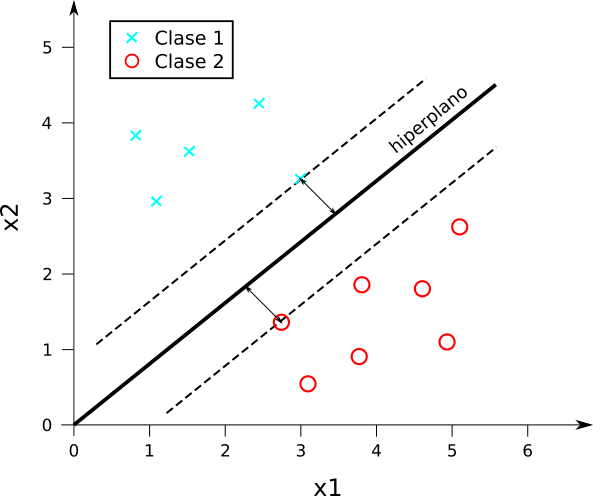
\includegraphics[width=9cm]{figs/svm_hiperplano.png}
  \end{center}
  \caption{Hiperplano de separación óptimo entre\\
            los datos de dos clases.}
  \label{fig:svm_hiperplano}
\end{figure}

El ejemplo de la Figura \ref{fig:svm_hiperplano} es separable linealmente (usando como hiperplano una línea), pero en la práctica real es complicado que esto suceda. Entonces, se hace uso de lo que se denomina \textit{kernel}, para transformar el conjunto de datos a un nuevo conjunto de una dimensión mayor, y que de esta manera se puedan separar linealmente en su nueva dimensión.

\subsection{K Vecinos más Cercanos (KNN)}

El \textit{K Vecinos más Cercanos} o KNN (K-Nearest Neighbours) es un algoritmo de aprendizaje supervisado utilizado para resolver tareas de clasificación. A diferencia de otros métodos, este utiliza siempre el conjunto de entrenamiento completo para realizar predicciones, en vez de crear un modelo en base a la relación de las entradas y las salidas. Es por ello, que es un método costoso computacionalmente para conjuntos de datos muy grades, pero ese no es nuestro caso.\\

El método está basado en calcular la distancia del dato a evaluar respecto a los demás datos. Partiendo de eso, el algoritmo se queda con los \textit{k} datos más cercanos, siendo \textit{k} un parámetro personalizable, y de estos elige la clase que más se repite, siendo esta la predicción realizada (Figura \ref{fig:knn}). Para medir la distancia entre datos, el método utilizado en este trabajo es el de distancia Euclídea (Ecuación \ref{ec:d_euclidea}).\\

\begin{figure} [h!]
  \begin{center}
    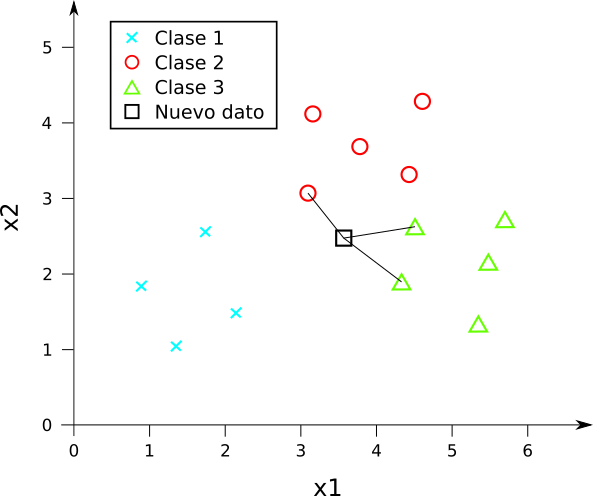
\includegraphics[width=9cm]{figs/knn.png}
  \end{center}
  \captionsetup{justification=centering}
  \caption{Ejemplo de KNN con $k = 3$.}
  \label{fig:knn}
\end{figure}

\begin{myequation}[h]
\begin{equation}
d(x^{\prime}, x^{(i)}) = \sqrt{\sum_{r=1}^{p}(x_{r}^{\prime}-x_{r}^{(i)})^{2}}
\nonumber
\label{ec:d_euclidea}
\end{equation}
\captionsetup{justification=centering}
\caption[Distancia Euclídea de un vector $x^{\prime}$ con \textit{p} características respecto al vector i-ésimo $(x^{(i)})$]{Distancia Euclídea de un vector $x^{\prime}$ \\
con \textit{p} características respecto al vector i-ésimo $(x^{(i)})$}
\end{myequation} 

\subsection{Redes Neuronales Multicapa}

Una red neuronal (Figura \ref{fig:red_neuronal}) es un modelo computacional inspirado en el funcionamiento del cerebro humano utilizado, en la mayoría de los casos, como técnica de aprendizaje supervisado. Está compuesta por un conjunto de neuronas que a su vez, si la red es multicapa, forman capas de neuronas. Realizo la excepción anterior porque existen también redes neuronales de una sola capa, denominadas perceptrón.\\

\begin{figure} [h!]
  \begin{center}
    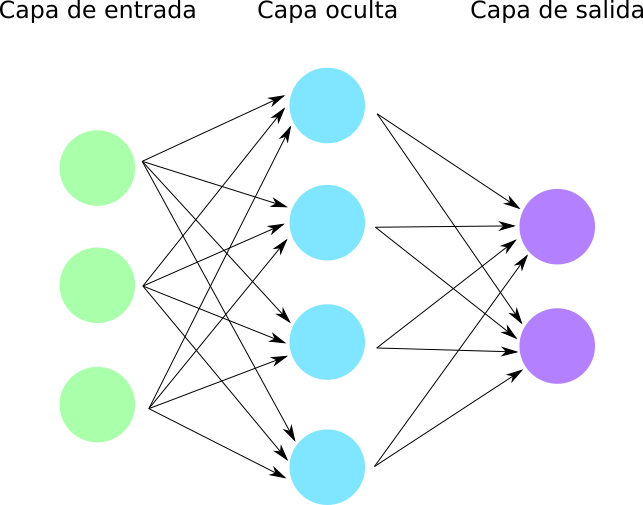
\includegraphics[width=11cm]{figs/redes_neuronales.png}
  \end{center}
  \caption{Red neuronal de tres capas y ocho neuronas.}
  \label{fig:red_neuronal}
\end{figure}

Todas las neuronas están interconectadas entre sí y cada una de esas neuronas estará formada por una función de decisión o función de transferencia (normalmente una función escalón, lineal o sigmoide). En el caso de una neurona de una sola entrada, la función de decisión evaluará la suma del producto del peso \textit{w} y la entrada \textit{x}, más el término independiente \textit{b} (Figura \ref{fig:neurona}).\\

\begin{figure} [h!]
  \begin{center}
    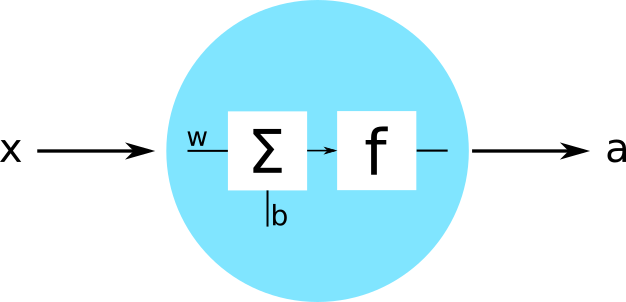
\includegraphics[width=8cm]{figs/neurona.png}
  \end{center}
  \captionsetup{justification=centering}
  \caption{Ejemplo del interior de una neurona de una entrada,\\
  donde \textit{x} es la entrada y \textit{a} es la salida.}
  \label{fig:neurona}
\end{figure}

La etapa de \textit{entrenamiento}, será un proceso iterativo en el que la red neuronal ajustará los valores de los pesos \textit{w} de cara a estimar el valor de salida.  Una vez que se haya finalizado el entrenamiento, la red se usa como una \textit{caja negra}, esto es, se le proporcionan una serie de entradas y te devuelve unas respectivas salidas, sin nosotros conocer lo que ha sucedido dentro.

\section{ROS (Robot Operating System)}

ROS (Robot Operating System)\footnote{ROS: \url{https://www.ros.org/}} (Figura \ref{fig:logo_ros}) es un \textit{middleware} para el desarrollo de software en robots, es decir, una colección de librerías software que proporcionan servicios tales como la abstracción del hardware o paso de mensajes entre procesos. Además, todo es código libre y multiplataforma (Linux, Windows, macOS).\\

\begin{figure} [h!]
  \begin{center}
    \includegraphics[width=5cm]{figs/ros_logo.png}
  \end{center}
  \captionsetup{justification=centering}
  \caption{Logo de ROS.}
  \label{fig:logo_ros}
\end{figure}

Cada uno de los procesos de ROS se denominan \textit{nodos} y se comunican entre sí usando \textit{topics}, ya sea en la misma máquina o de forma remota en una red local. El envío y recibimiento de mensajes a través de los \textit{topics}, se consigue haciendo uso de publicadores y subscriptores. Además, ofrece otras opciones de comunicación como los servicios o acciones. El nodo \textit{máster} será el encargado de permitir que todos los nodos se localicen entre sí, proporcionando ---entre otras cosas--- servicios de \textit{naming}. En la Figura \ref{fig:ros} se puede observar un esquema reducido de lo que sería una comunicación entre un nodo publicador y un nodo suscriptor a través del \textit{topic} \verb|\ejemplo|.\\

\begin{figure} [h!]
  \begin{center}
    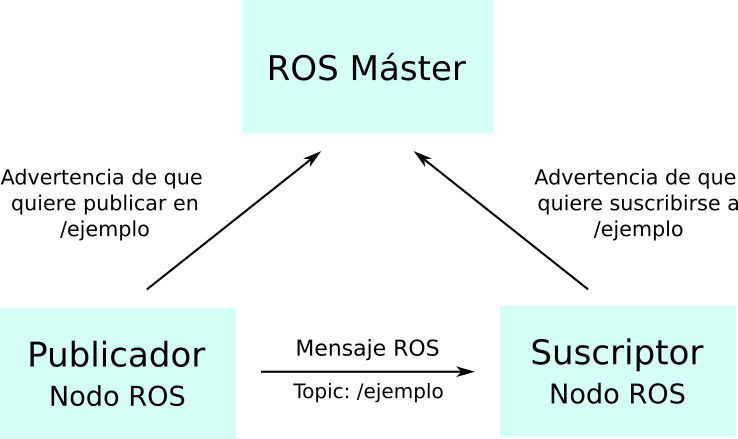
\includegraphics[width=11cm]{figs/ros.png}
  \end{center}
  \captionsetup{justification=centering}
  \caption{Esquema simple de una comunicación publicador-suscriptor en ROS.}
  \label{fig:ros}
\end{figure}

Existe una gran comunidad de usuarios desarrolladores que aportan paquetes al entorno ROS y, por lo tanto, lo hacen aún más rico. Entre todos estos paquetes, podemos encontrar algunos enfocados en ---por ejemplo--- identificación de objetos o reconocimiento de voz. La versión de ROS usada en este trabajo será ROS Noetic y el resultado final del sistema será de código libre para dicha comunidad de ROS.